%  LaTeX support: latex@mdpi.com 
%  For support, please attach all files needed for compiling as well as the log file, and specify your operating system, LaTeX version, and LaTeX editor.

%=================================================================
\documentclass[cancers,article,submit,moreauthors,pdftex]{Definitions/mdpi} 

% For posting an early version of this manuscript as a preprint, you may use "preprints" as the journal and change "submit" to "accept". The document class line would be, e.g., \documentclass[preprints,article,accept,moreauthors,pdftex]{mdpi}. This is especially recommended for submission to arXiv, where line numbers should be removed before posting. For preprints.org, the editorial staff will make this change immediately prior to posting.

%--------------------
% Class Options:
%--------------------
%----------
%journal Cancers
%----------
% Choose between the following MDPI journals:
% acoustics, actuators, addictions, admsci, adolescents, aerospace, agriculture, agriengineering, agronomy, ai, algorithms, allergies, analytica, animals, antibiotics, antibodies, antioxidants, appliedchem, applmech, applmicrobiol, applnano, applsci, arts, asi, atmosphere, atoms, audiolres, automation, axioms, batteries, bdcc, behavsci, beverages, biochem, bioengineering, biologics, biology, biomechanics, biomedicines, biomedinformatics, biomimetics, biomolecules, biophysica, biosensors, biotech, birds, bloods, brainsci, buildings, businesses, cancers, carbon, cardiogenetics, catalysts, cells, ceramics, challenges, chemengineering, chemistry, chemosensors, chemproc, children, civileng, cleantechnol, climate, clinpract, clockssleep, cmd, coatings, colloids, compounds, computation, computers, condensedmatter, conservation, constrmater, cosmetics, crops, cryptography, crystals, curroncol, cyber, dairy, data, dentistry, dermato, dermatopathology, designs, diabetology, diagnostics, digital, disabilities, diseases, diversity, dna, drones, dynamics, earth, ebj, ecologies, econometrics, economies, education, ejihpe, electricity, electrochem, electronicmat, electronics, encyclopedia, endocrines, energies, eng, engproc, entropy, environments, environsciproc, epidemiologia, epigenomes, fermentation, fibers, fire, fishes, fluids, foods, forecasting, forensicsci, forests, fractalfract, fuels, futureinternet, futuretransp, futurepharmacol, futurephys, galaxies, games, gases, gastroent, gastrointestdisord, gels, genealogy, genes, geographies, geohazards, geomatics, geosciences, geotechnics, geriatrics, hazardousmatters, healthcare, hearts, hemato, heritage, highthroughput, histories, horticulturae, humanities, hydrogen, hydrology, hygiene, idr, ijerph, ijfs, ijgi, ijms, ijns, ijtm, ijtpp, immuno, informatics, information, infrastructures, inorganics, insects, instruments, inventions, iot, j, jcdd, jcm, jcp, jcs, jdb, jfb, jfmk, jimaging, jintelligence, jlpea, jmmp, jmp, jmse, jne, jnt, jof, joitmc, jor, journalmedia, jox, jpm, jrfm, jsan, jtaer, jzbg, kidney, land, languages, laws, life, liquids, literature, livers, logistics, lubricants, machines, macromol, magnetism, magnetochemistry, make, marinedrugs, materials, materproc, mathematics, mca, measurements, medicina, medicines, medsci, membranes, metabolites, metals, metrology, micro, microarrays, microbiolres, micromachines, microorganisms, minerals, mining, modelling, molbank, molecules, mps, mti, nanoenergyadv, nanomanufacturing, nanomaterials, ncrna, network, neuroglia, neurolint, neurosci, nitrogen, notspecified, nri, nursrep, nutrients, obesities, oceans, ohbm, onco, oncopathology, optics, oral, organics, osteology, oxygen, parasites, parasitologia, particles, pathogens, pathophysiology, pediatrrep, pharmaceuticals, pharmaceutics, pharmacy, philosophies, photochem, photonics, physchem, physics, physiolsci, plants, plasma, pollutants, polymers, polysaccharides, proceedings, processes, prosthesis, proteomes, psych, psychiatryint, publications, quantumrep, quaternary, qubs, radiation, reactions, recycling, regeneration, religions, remotesensing, reports, reprodmed, resources, risks, robotics, safety, sci, scipharm, sensors, separations, sexes, signals, sinusitis, smartcities, sna, societies, socsci, soilsystems, solids, sports, standards, stats, stresses, surfaces, surgeries, suschem, sustainability, symmetry, systems, taxonomy, technologies, telecom, textiles, thermo, tourismhosp, toxics, toxins, transplantology, traumas, tropicalmed, universe, urbansci, uro, vaccines, vehicles, vetsci, vibration, viruses, vision, water, wevj, women, world 

%---------
% article
%---------
% The default type of manuscript is "article", but can be replaced by: 
% abstract, addendum, article, book, bookreview, briefreport, casereport, comment, commentary, communication, conferenceproceedings, correction, conferencereport, entry, expressionofconcern, extendedabstract, datadescriptor, editorial, essay, erratum, hypothesis, interestingimage, obituary, opinion, projectreport, reply, retraction, review, perspective, protocol, shortnote, studyprotocol, systematicreview, supfile, technicalnote, viewpoint, guidelines, registeredreport, tutorial
% supfile = supplementary materials

%----------
% submit
%----------
% The class option "submit" will be changed to "accept" by the Editorial Office when the paper is accepted. This will only make changes to the frontpage (e.g., the logo of the journal will get visible), the headings, and the copyright information. Also, line numbering will be removed. Journal info and pagination for accepted papers will also be assigned by the Editorial Office.

%------------------
% moreauthors
%------------------
% If there is only one author the class option oneauthor should be used. Otherwise use the class option moreauthors.

%---------
% pdftex
%---------
% The option pdftex is for use with pdfLaTeX. If eps figures are used, remove the option pdftex and use LaTeX and dvi2pdf.


%%%%%%%%%%%%%%%%%%%%%%%%%%%%%%%%%% Tex
%\usepackage[bf]{caption}
%\newcommand{\bcaption}[2]{\caption{\textbf{#1} #2}}

%\usepackage[upplemac]{inputenc} %applemac support if unicode package fails
%\usepackage[latin1]{inputenc} %UNIX support if unicode package fails
%...
%\usepackage{graphicx}
%\DeclareGraphicsExtensions{.pdf,.png} % for high-resolution PDF image
%\usepackage{hyperref}
%\usepackage{url}

\usepackage{array}
\usepackage{ragged2e}
\usepackage{rotating}
% \usepackage{array}
\usepackage{multirow}
\usepackage{colortbl}
\usepackage{hhline}
\usepackage{siunitx} % for  1e-10 scientific notation
%\usepackage{caption}
%\usepackage{subcaption}
\usepackage{booktabs, multirow} % for borders and merged ranges
\usepackage{soul}% for underlines
%\usepackage[table]{xcolor} % for cell colors
\usepackage{changepage,threeparttable} 

%%% for abbreviations, or acronyms
\usepackage[automake, acronym, nopostdot]{glossaries} 
\usepackage{glossary-inline}
%\setacronymstyle{long-short}
%\renewcommand*{\glossarysection}[2][]{} 
%\renewcommand*{\glossarysection}[2][]{\textbf{#1}: }
% for abbreviations environment
%\newcommand{\abbrlabel}[1]{\makebox[3cm][l]{\textbf{#1}\ \dotfill}}
\newenvironment{abbreviation}%{\begin{list}{}{\renewcommand{\makelabel}{\abbrlabel}}}{\end{list}}
% \newenvironment{<name>}[<number>][<default>]


\makeglossaries %https://tex.stackexchange.com/questions/110095/list-of-acronyms-is-not-displayed
\newacronym{fdr}{FDR}{false discovery rate}

\newacronym{hpa}{HPA}{the Human Protein Atlas}
\newacronym{hnscc}{HNSCC}{head and neck squamous cell carcinoma}
\newacronym{tcga}{TCGA}{the Cancer Genome Atlas}
\newacronym{tcpa}{TCPA}{the Cancer Proteome Atlas}
\newacronym{rna}{RNA}{ribonucleic acid}
\newacronym{rnaseq}{RNA-Seq}{RNA sequencing}
\newacronym{lncrna}{lncRNA}{long non-coding RNA}
%\newacronym{km}{KM}{Kaplan-Meier}
\newacronym{rppa}{RPPAs}{reverse-phase protein arrays}
\newacronym{rpma}{RPMA}{reverse-phase protein lysate microarray}

\newacronym{mmp}{MMP}{matrix metalloproteinase}
 %DKK1, CAMK2N1, STC2, PGK1, SURF4, USP10, NDFIP1, FOXA2, STIP1, and DKC1
 %ZNF557, ZNF266, IL19, MYO1H, FCGBP, LOC148709, EVPLL, PNMA5, KIAA1683, and NPB

\newacronym{DKK1}{DKK1}{dickkopf WNT signaling pathway inhibitor 1} 
\newacronym{CAMK2N1}{CAMK2N1}{calcium/calmodulin dependent protein kinase II inhibitor 1} 
\newacronym{STC2}{STC2}{stanniocalcin 2} 
\newacronym{PGK1}{PGK1}{phosphoglycerate kinase 1} 
\newacronym{SURF4}{SURF4}{surfeit 4} 
\newacronym{USP10}{USP10}{ubiquitin specific peptidase 10} 
\newacronym{NEDD4}{NEDD4}{neural precursor cell expressed, developmentally down-regulated 4}
\newacronym{NDFIP1}{NDFIP1}{NEDD4 family interacting protein 1} 
\newacronym{FOXA2}{FOXA2}{forkhead box A2} 
\newacronym{STIP1}{STIP1}{stress-induced-phosphoprotein 1} 
\newacronym{DKC1}{DKC1}{dyskeratosis congenita 1, dyskerin} 

\newacronym{ZNF557}{ZNF557}{zinc finger protein 557} 
\newacronym{ZNF266}{ZNF266}{zinc finger protein 266} 
\newacronym{IL19}{IL19}{interleukin 19} 
\newacronym{MYO1H}{MYO1H}{myosin 1H} 
\newacronym{FCGBP}{FCGBP}{Fc fragment of IgG binding protein} 
\newacronym{LOC148709}{LOC148709}{LncRNA LOC148709} 
\newacronym{EVPLL}{EVPLL}{envoplakin-like protein} 
\newacronym{PNMA5}{PNMA5}{paraneoplastic antigen like 5} 
%\newacronym{KIAA1683}{KIAA1683}{IQCN, IQ Motif Containing N} 
\newacronym{IQCN}{IQCN}{IQ motif containing N} % previous name KIAA1683
% "IQ" refers to the first two amino acids of the motif: isoleucine (commonly) and glutamine (invariably)
\newacronym{NPB}{NPB}{neuropeptide B} 

 \newacronym{rt}{RT}{radiation therapy}
 \newacronym{nccn}{NCCN}{National Comprehensive Cancer Network}
 \newacronym{hif}{HIF}{hypoxia-inducible factor}
 \newacronym{egfr}{EGFR}{epidermal growth factor receptor}
 \newacronym{ras}{RAS}{rat sarcoma}
 \newacronym{hras}{HRAS}{Harvey rat sarcoma viral oncoprotein}
 \newacronym{erk}{ERK}{extracellular signal-regulated kinases}
 \newacronym{us}{US}{United States}
 \newacronym{fda}{FDA}{Food and Drug Administration}
 \newacronym{tpf}{Tax-PF}{docetaxel, cisplatin, and 5-fluorouracil}
 \newacronym{tki}{TKI}{tyrosine kinase inhibitor}
 \newacronym{her}{HER}{human epidermal growth factor receptor}
 \newacronym{ici}{ICI}{immune-checkpoint inhibitor}
 \newacronym{ctla4}{CTLA-4}{cytotoxic T lymphocyte antigen 4}
 \newacronym{pd1}{PD-1}{programmed death 1}
 \newacronym{pdl1}{PD-L1}{programmed death ligand 1}
 \newacronym{tim3}{TIM-3}{T-cell immunoglobulin mucin protein 3}
 \newacronym{lag3}{LAG-3}{lymphocyte activation gene 3}
 \newacronym{ifng}{IFN-$\gamma$}{interferon gamma}
 \newacronym{tigit}{TIGIT}{T cell immunoglobin and immunoreceptor tyrosine-based inhibitory motif}
 \newacronym{gitr}{GITR}{glucocorticoid-induced tumor necrosis factor receptor}
 \newacronym{vista}{VISTA}{V-domain Ig suppressor of T-cell activation}
 \newacronym{tmsb4x}{TMSB4X}{thymosin beta-4 X-linked}
 \newacronym{emt}{EMT}{epithelial-mesenchymal-transition}
 \newacronym{gdc}{GDC}{Genomic Data Commons}
 \newacronym{nci}{NCI}{the National Cancer Institute}
 \newacronym{gdac}{GDAC}{Genome Data Analysis Center}
 \newacronym{rest}{REST}{Representational State Transfer} 
 \newacronym{api}{API}{Application Programmable Interface}
\newacronym{grch38}{GRCh38}{Genome Reference Consortium Homo sapiens genome assembly 38}
\newacronym{fpkm}{FPKM}{Fragments per kilobase per million reads mapped}
\newacronym{rsem}{RSEM}{RNA-Seq by Expectation-Maximization}
\newacronym{slca}{SLC35E2A}{solute carrier family 35 member E2A}
\newacronym{slcb}{SLC35E2B}{solute carrier family 35 member E2B}
\newacronym{cde}{CDE}{Common Data Element}
\newacronym{id}{ID}{identification}
\newacronym{ajcc}{AJCC}{the American Joint Committee on Cancer}
\newacronym{uicc}{UICC}{he Union for International Cancer Control}
\newacronym{tnm}{TNM}{the tumor size (T), cervical lymph node metastases (N), and distal metastasis status (M)}
\newacronym{ci95}{95\% CI}{95\% confidence interval}
\newacronym{os}{OS}{overall survival}
\newacronym{hr}{HR}{hazard ratio}
\newacronym{hpv}{HPV}{human papillomavirus}
\newacronym{ene}{ENE}{extra-nodal extension}
\newacronym{lvsi}{LVSI}{lymph-vascular space invasion}
\newacronym{pni}{PNI}{perineural invasion}
\newacronym{doi}{DOI}{depth of invasion}
\newacronym{lnd}{LND}{lymph node density}
\newacronym{wpoi5}{WPOI-5}{worst pattern of invasion score 5}
\newacronym{glut4}{GLUT4}{glucose transporters 4}
\newacronym{slc2a4}{SLC2A4}{solute carrier family 2 member A4}
\newacronym{trim24}{TRIM24}{tripartite motif-containing 24}
\newacronym{til}{TIL}{tumor-infiltrating lymphocytes}
\newacronym{tmb}{TMB}{tumor mutational burden}


%=================================================================
\firstpage{1} 
\makeatletter 
\setcounter{page}{\@firstpage} 
\makeatother
\pubvolume{1}
\issuenum{1}
\articlenumber{0}
\pubyear{2021}
\copyrightyear{2021}
%\externaleditor{Academic Editor: Firstname Lastname}
\datereceived{} 
\dateaccepted{} 
\datepublished{} 

%------------------------------------------------------------------
% The following line should be uncommented if the LaTeX file is uploaded to arXiv.org
%\pdfoutput=1

%=================================================================
% Add packages and commands here. The following packages are loaded in our class file: fontenc, inputenc, calc, indentfirst, fancyhdr, graphicx, epstopdf, lastpage, ifthen, lineno, float, amsmath, setspace, enumitem, mathpazo, booktabs, titlesec, etoolbox, tabto, xcolor, soul, multirow, microtype, tikz, totcount, changepage, paracol, attrib, upgreek, cleveref, amsthm, hyphenat, natbib, hyperref, footmisc, url, geometry, newfloat, caption

%=================================================================
%% Please use the following mathematics environments: Theorem, Lemma, Corollary, Proposition, Characterization, Property, Problem, Example, ExamplesandDefinitions, Hypothesis, Remark, Definition, Notation, Assumption
%% For proofs, please use the proof environment (the amsthm package is loaded by the MDPI class).

%=================================================================
% Full title of the paper (Capitalized)
\Title{A Global Genome-wide Scan with Optimal Cutoff Mining for Emerging Biomarkers in Head and Neck Squamous Cell Carcinoma}

% MDPI internal command: Title for citation in the left column
\TitleCitation{A Global Genome-wide Scan with Optimal Cutoff Mining for Emerging Biomarkers in Head and Neck Squamous Cell Carcinoma}

% Author Orchid ID: enter ID or remove command
\newcommand{\orcidauthorA}{0000-0002-4476-2600} % Add \orcidA{} behind the author's name
\newcommand{\orcidauthorB}{0000-0001-6497-4232} % Add \orcidB{} behind the author's name

% Authors, for the paper (add full first names)
\Author{
Li-Hsing Chi $^{1,2}$\orcidA{}, Alexander TH Wu $^{1}$,
Michael Hsiao $^{3}$*
and Yu-Chuan (Jack) Li $^{1,4}$*\orcidB{}}
%\Author{Firstname Lastname $^{1,\dagger,\ddagger}$\orcidA{}, Firstname Lastname $^{1,\ddagger}$ and Firstname Lastname $^{2,}$*}

% MDPI internal command: Authors, for metadata in PDF
\AuthorNames{Li-Hsing Chi, Alexander TH Wu, Michael Hsiao and Yu-Chuan (Jack) Li}

% MDPI internal command: Authors, for citation in the left column
\AuthorCitation{Chi, LH.; Wu, ATH.; Hsiao, M.; Li, YCJ.}

% Affiliations / Addresses (Add [1] after \address if there is only one affiliation.)
\address{%
$^{1}$ \quad The Ph.D. Program for Translational Medicine, College of Medical Science and Technology\unskip, 
    Taipei Medical University and Academia Sinica\unskip, Taipei\unskip, Taiwan\\
$^{2}$ \quad Division of Oral and Maxillofacial Surgery, Department of Dentistry\unskip,
    Taipei Medical University Hospital\unskip, Taipei\unskip, Taiwan\\
$^{3}$ \quad Genomics Research Center\unskip, 
    Academia Sinica\unskip, Taipei\unskip, Taiwan\\
$^{4}$ \quad Graduate Institute of Biomedical Informatics, College of Medical Science and Technology\unskip, Taipei Medical University\unskip, Taipei\unskip, Taiwan\\
}

% Contact information of the corresponding author
\corres{Correspondence: Hsiao: mhsiao@gate.sinica.edu.tw; Li: jaak88@gmail.com}
%(optional; include country code; if there are multiple corresponding authors, add author initials) +xx-xxxx-xxx-xxxx (F.L.)}

% Current address and/or shared authorship
%\firstnote{Current address: Affiliation 3} 
%\secondnote{These authors contributed equally to this work.}
% The commands \thirdnote{} till \eighthnote{} are available for further notes

%\simplesumm{} % Simple summary

%\conference{} % An extended version of a conference paper

% Abstract (Do not insert blank lines, i.e. \\) 
\abstract{The survival analysis of the Cancer Genome Atlas (TCGA) dataset is a well-known method to discover the gene expression-based prognostic biomarkers of head and neck squamous cell carcinoma (HNSCC). It is necessary to determine a cutoff point by the patients' dichotomization for the continuous gene expression in survival analysis. There is some optimization software for cutoff determination. However, the software's predetermined cutoffs are usually set at the median or quantiles of RNA sequencing value to perform the survival analyses. There are few clinicopathological features available on their pre-processed data sets.
We developed a comprehensive workflow that includes data retrieving and pre-processing, feature selection, cutoff mining engine, Kaplan-Meier survival analysis, Cox proportional hazard modeling, and biomarker discovery.
Using this workflow on the TCGA HNSCC cohort, we scanned human protein-coding genes. After adjustment with confounders and Bonferroni adjusted P-value, ten candidate biomarkers, named as DKK1, CAMK2N1, STC2, PGK1, SURF4, USP10, NDFIP1, FOXA2, STIP1, and DKC1, are significantly associated with the poor prognosis of overall survival. At the same time, the other ten genes were over-expressed in the better survival patients, named as ZNF557, ZNF266, IL19, MYO1H, FCGBP, LOC148709, EVPLL, PNMA5, IQCN (previous name as KIAA1683), and NPB.
We suggest this workflow could help for biomarker discovery.}

% Keywords
\keyword{Head and Neck Squamous Cell Carcinoma (HNSCC);
%Genome Database\sep
the Cancer Genome Atlas (TCGA);
RNA-sequencing;
Survival Analysis;
Optimal Cutoff;
%Biomarker\sep % Discovery\sep
%Tumor Type-agnostic Therapy\sep
%Immuno-Oncology\sep
%Targeted Therapy\sep
%Systemic Therapy\sep
Surgical Margin} 

% The fields PACS, MSC, and JEL may be left empty or commented out if not applicable
%\PACS{J0101}
%\MSC{}
%\JEL{}

%%%%%%%%%%%%%%%%%%%%%%%%%%%%%%%%%%%%%%%%%%
% Only for the journal Diversity
%\LSID{\url{http://}}

%%%%%%%%%%%%%%%%%%%%%%%%%%%%%%%%%%%%%%%%%%
% Only for the journal Applied Sciences:
%\featuredapplication{Authors are encouraged to provide a concise description of the specific application or a potential application of the work. This section is not mandatory.}
%%%%%%%%%%%%%%%%%%%%%%%%%%%%%%%%%%%%%%%%%%

%%%%%%%%%%%%%%%%%%%%%%%%%%%%%%%%%%%%%%%%%%
% Only for the journal Data:
%\dataset{DOI number or link to the deposited data set in cases where the data set is published or set to be published separately. If the data set is submitted and will be published as a supplement to this paper in the journal Data, this field will be filled by the editors of the journal. In this case, please make sure to submit the data set as a supplement when entering your manuscript into our manuscript editorial system.}

%\datasetlicense{license under which the data set is made available (CC0, CC-BY, CC-BY-SA, CC-BY-NC, etc.)}

%%%%%%%%%%%%%%%%%%%%%%%%%%%%%%%%%%%%%%%%%%
% Only for the journal Toxins
%\keycontribution{The breakthroughs or highlights of the manuscript. Authors can write one or two sentences to describe the most important part of the paper.}

%%%%%%%%%%%%%%%%%%%%%%%%%%%%%%%%%%%%%%%%%%
% Only for the journal Encyclopedia
%\encyclopediadef{Instead of the abstract}
%\entrylink{The Link to this entry published on the encyclopedia platform.}
%%%%%%%%%%%%%%%%%%%%%%%%%%%%%%%%%%%%%%%%%%
% for Cancers
% *** All Figures, Schemes and Tables should be inserted into the main text close to their first citation
% https://www.mdpi.com/journal/cancers/instructions#preparation

\begin{document}
%%%%%%%%%%%%%%%%%%%%%%%%%%%%%%%%%%%%%%%%%%
%\setcounter{section}{-1} %% Remove this when starting to work on the template.
%\section{How to Use this Template}

%The template details the sections that can be used in a manuscript. Note that the order and names of article sections may differ from the requirements of the journal (e.g., the positioning of the Materials and Methods section). Please check the instructions on the authors' page of the journal to verify the correct order and names. For any questions, please contact the editorial office of the journal or support@mdpi.com. For LaTeX-related questions please contact latex@mdpi.com.
%The order of the section titles is: Introduction, Materials and Methods, Results, Discussion, Conclusions for these journals: aerospace,algorithms,antibodies,antioxidants,atmosphere,axioms,biomedicines,carbon,crystals,designs,diagnostics,environments,fermentation,fluids,forests,fractalfract,informatics,information,inventions,jfmk,jrfm,lubricants,neonatalscreening,neuroglia,particles,pharmaceutics,polymers,processes,technologies,viruses,vision

\section{Introduction}

Head and neck squamous cell carcinoma (\acrshort{hnscc}), including oral, oropharyngeal, and hypopharyngeal origin, is the fourth leading cancer causes of death for males in Taiwan\cite{MOHW_death2017}. The age-standardized incidence rate of \acrshort{hnscc} in males is 42.43 per 100,000 persons\cite{MOHW_incidence2018}. 
% chemotherapy => systemic therapy
The treatment strategies of \acrshort{hnscc} are surgery alone, systemic therapy with concurrent radiation therapy (systemic therapy/\acrshort{rt}), or surgery with adjuvant systemic therapy/\acrshort{rt} (according to \acrlong{nccn}, \acrshort{nccn} Clinical Practice Guidelines in \acrshort{hnscc}, Version 2.2020)\cite{Pfister2020a}. Despite the improvement in those interventions, the survival of \acrshort{hnscc} has improved only marginally over the past decade worldwide\cite{hpa2019}. The critical advancement of targeted therapy and immuno-oncology should benefit from emerging prognostic biomarkers, which guide the development of modern systemic therapy.

%% TP53 gene => p53 protein; mutation of TP53
Accumulative knowledge showed that some biomarkers have prognostic significance in \acrshort{hnscc}. For example, node-negative \acrshort{hnscc} patients with p53 overexpression were found to have lower survival\cite{DeVicente2004}.
Overexpression of \acrfull{hif}-1 alpha\cite{Aebersold2001} or Ki-67\cite{Couture2002} was found to be correlated with poor response to radiotherapy of \acrshort{hnscc}. The \acrfull{egfr}\cite{O-Charoenrat2000}\cite{Bentzen2005} and \acrfull{mmp}\cite{Harrington2017} were found to be over-expressed to promote invasion and metastasis of \acrshort{hnscc}.
From 2000 to 2006, the anti-\acrshort{egfr} antibody-drug (cetuximab) has been developed and combined with radiotherapy, known as bio-\acrshort{rt}, to increase survival of unresectable locoregionally advanced disease\cite{Bonner2006a}.
The systemic therapy of cetuximab plus platinum-fluorouracil chemotherapy (EXTREME regimen) improves overall survival when given as first-line treatment in patients with recurrent or metastatic \acrshort{hnscc}\cite{Vermorken2008}\cite{Rivera2009}. It was approved by the \acrshort{us} \acrfull{fda} in 2008. In advance, the bio-\acrshort{rt} could have proceeded with \acrfull{tpf} induction chemotherapy to overcome the radio-resistance of \acrshort{hnscc}\cite{Blanchard2013}.

However, Rampias and his colleagues suggested \acrfull{hras} mutations could mediate cetuximab resistance in systemic therapy of \acrshort{hnscc} via the \acrshort{egfr}/\acrfull{ras}/\acrfull{erk} signaling pathway\cite{Rampias2014}.
After that, the \acrshort{egfr} \acrfull{tki} was introduced to help cetuximab in 2018. The anti-tumor activity was observed in a phase 1 trial for \acrshort{hnscc} patients using cetuximab and afatinib, a \acrshort{tki} of \acrshort{egfr}, \acrfull{her}2, and \acrshort{her}4\cite{Gazzah2018}. Other \acrshort{egfr} \acrshort{tki}, such as gefitinib, erlotinib, osimertinib, were also developed to treat advanced \acrshort{hnscc}.
Although 90\% of \acrshort{hnscc} has overexpression of \acrshort{egfr}, cetuximab has only 10\% to 20\% response rate on those patients. So far, cetuximab is still the only drug of choice with proven efficacy, which targeted the selected \acrshort{hnscc} patients\cite{Taberna2019}.

Until the immuno-oncology era, \acrfull{ici} was introduced since 2014 for treating \acrshort{hnscc}\cite{Seiwert2014}\cite{Swanson2015}.
The \acrshort{ici} works on immune checkpoint molecules, which including \acrfull{pd1}, \acrfull{ctla4}, \acrfull{tim3}, \acrfull{lag3}, \acrfull{tigit}, \acrfull{gitr} and \acrfull{vista}\cite{Mei2020}.
The \acrshort{us} \acrshort{fda} has approved the anti-\acrshort{pd1} agents, pembrolizumab, and nivolumab, as a monotherapy for the platinum-treated patients of recurrent or metastatic \acrshort{hnscc}\cite{Cramer2019}. However, because of the complexity of immune-tumor interaction, \acrshort{ici} has not to guarantee the response to \acrfull{pdl1} expressed \acrshort{hnscc}\cite{Swanson2015}.
According to the phase 3 KEYNOTE-048 study, \acrshort{pdl1} is a validated biomarker used in clinical guidance for candidate selection of pembrolizumab\cite{Burtness2019}\cite{Gavrielatou2020}.

In our previous proteomic study in 2017, \acrfull{tmsb4x} was reported to be related to tumor growth and metastasis of \acrshort{hnscc}\cite{Chi2017}. It was also found by the subsequent investigations that \acrshort{tmsb4x} engaged in tumor aggressiveness through \acrfull{emt} on pancreatic\cite{Zhang2008}, gastric\cite{Ryu2012}, colorectal\cite{Gemoll2015}, lung\cite{Huang2016}, ovarian\cite{Chu2019} and melanoma\cite{Makowiecka2019} cancers. Thus, it might be suggested that \acrshort{tmsb4x}  is possible for tumor type-agnostic therapy\cite{Yan2018} as a common biomarker crossing several types of cancer.
%TMSB4X proteins regulate intracellular signal transduction and has been proved to overexpress in various cancers, including colorectal, lung, gastric, pancreatic, and squamous cell cancers.\cite{Chi2017}
% https://doi.org/10.1038/s41598-017-09539-w

In summary, identifying predictive biomarkers for selecting standard-of-care or advanced systemic therapy\cite{Cristina2019} in \acrshort{hnscc} is crucial. 
However, there are three challenges of biomarker discovery from survival analysis, so far.
Firstly, although \acrshort{tcga} genomics data were harmonized, there is unclean data, including null expressed genes, which over 50\% of the cohort, should be manually investigated and cleaned.
Second, we need to find a way to determine candidates from the expression level of 20,500 human protein-coding genes\cite{Clamp2007}. Usually, the investigators should get the rationale or revelation of the genes of interest on a specific cancer type. They should upload those genes manually onto bioinformatics tools, such as SurvExpress (http://bioinformatica.mty.itesm.mx:8080/Biomatec/ \newline
SurvivaX.jsp, which has been lost since Oct/2019 and currently out of funds), analyze with \acrshort{tcga} cohort. After downloading the survival results, they could curate plots and tables carefully.
It is not possible to scan the whole human protein-coding genome in this way.
Third, we need to find an optimal cutpoint of those \acrshort{rna} expression data to maximize candidate mining coverage. The above mentioned online tools might set a cutpoint at the median, 1/4 quantile, or 3/4 quantile for subsequent analyses. There are several visualization software or R packages which deal with cutoff determination, such as Prognoscan\cite{Mizuno2009a}, Cutoff Finder\cite{Budczies2012}, Findcut\cite{Chang2017a}, Human protein atlas\cite{Uhlen2017}, OptimalCutpoints\cite{Cristina2019},  cutpointr (available at https://github.com/thie1e/ \newline
cutpointr), and cutoffR (available at https://cran.r-project.org/web/
packages/cutoffR). However, non of them could combine the scanning of the protein-coding genes and cutoff optimization programmatically.

In our approach, this article described a comprehensive workflow implemented in the R script, which runs on the Rstudio server. Its functions include data retrieving and pre-processing, feature selection, cutoff mining engine, Kaplan-Meier survival analysis, Cox proportional hazard modeling, and biomarker selection.
Using this workflow on the \acrshort{tcga} \acrshort{hnscc} cohort, the 20,500 human protein-coding genes were scanned. The analysis workflow is shown in Figure \ref{fig:figure1}.
%We found that the surgical margin status and tobacco exposure are independent risk factors of patient survival. 
%Our findings also suggested several candidate biomarkers are associated with the prognosis of overall survival (OS) under optimal cutoff point with significant P-value. Those genes may be potential therapeutic targets of HNSCC.

%\subsubsection{Figure 1:h}
\begin{figure}[hp]
\centering
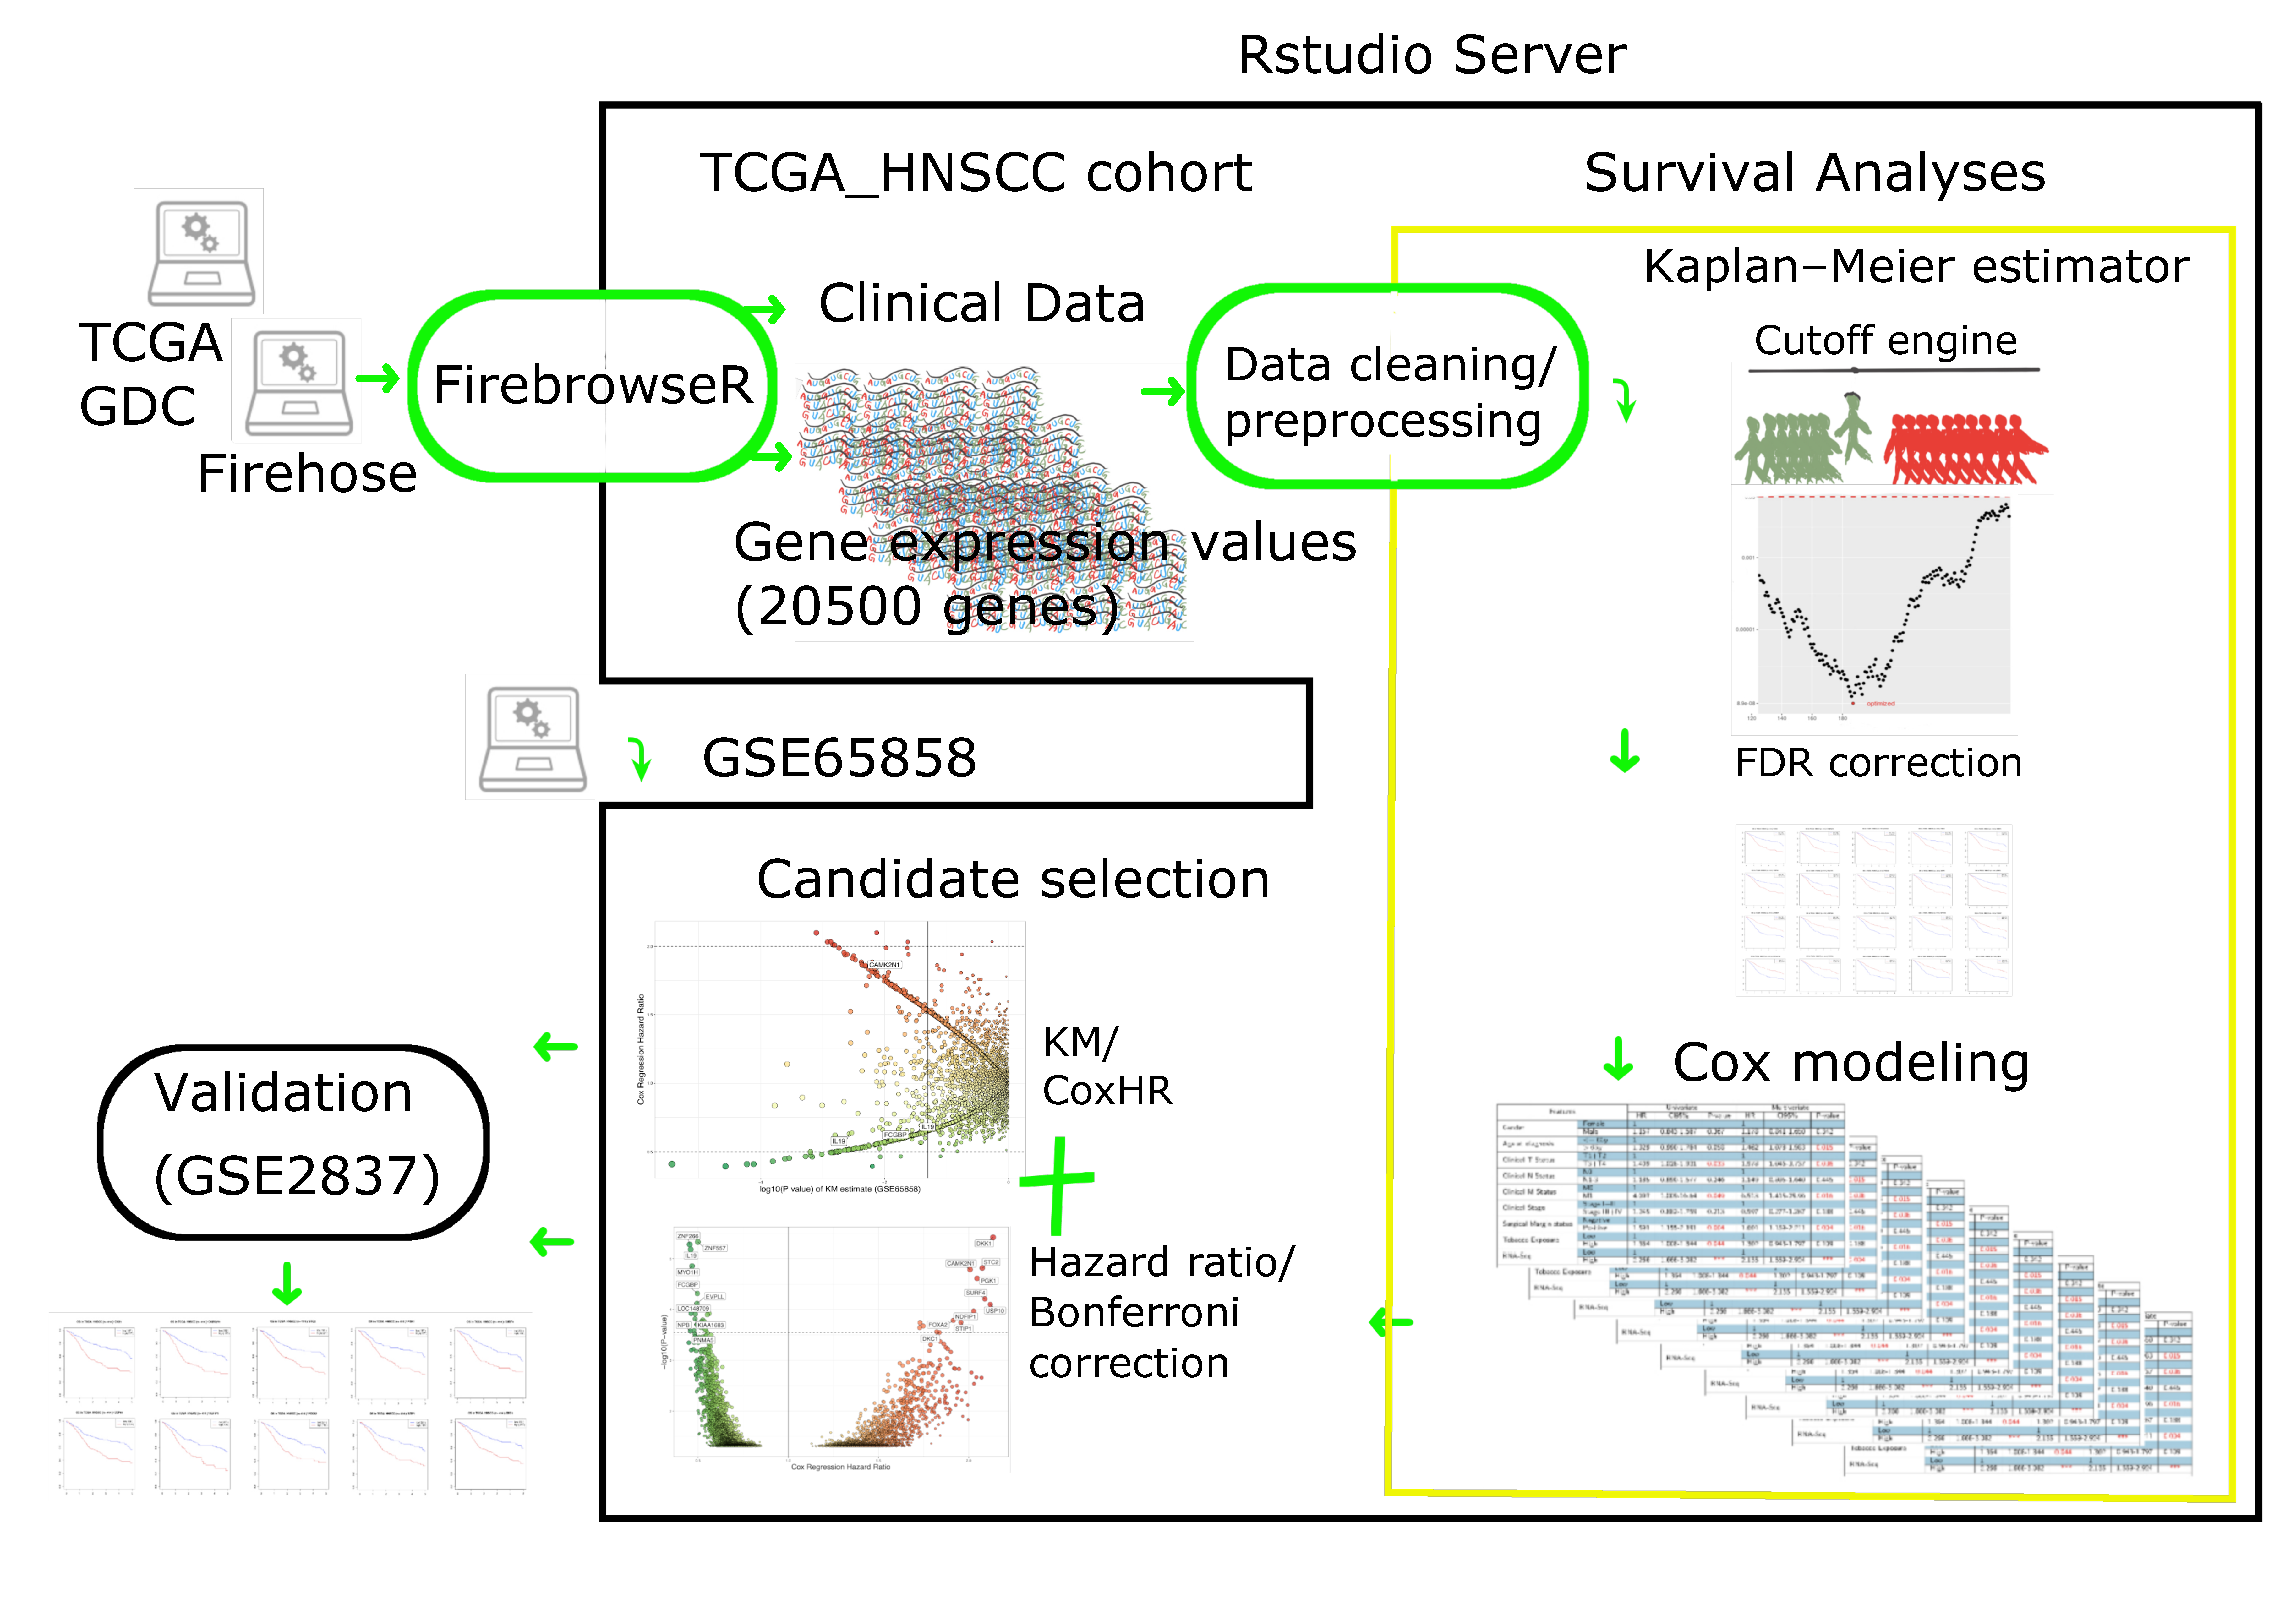
\includegraphics[width=14cm]{Figure_1_manuscript_workflow} % .PDF is better than .png
%, height=8cm
%\caption
\bcaption{A workflow of \acrshort{hnscc} biomarker discovery, step 1 (blue line: main procedure) and step 2 (orange line: analysis export).}
%Step 3 (purple line: dealing with surgical margin).
{The "main procedure" includes data retrieving from TCGA GDC data portal, data process with merging and cleaning, then performing the survival analyses. The Cutoff engine (cutofFinder\_func.HNSCC.R) might calculate all possible Kaplan-Meier P-value to find the optimal cutoff value of RNA-Seq for subsequent Cox modeling (a draft diagram shown on the upper right corner "HNSCC cohort", the serial cut for grouping patients with low [green] or high [red] expression of a specific gene, to yield a collection of P-values; please see Materials and Methods section for details). The step 2 "analysis export" performs dissecting and selection of candidate genes by Bonferroni adjusted P-value as well as a hazard ratio of Cox model, which was based on the results from the step 1.
(HNSCC: head and neck squamous cell carcinoma; TCGA: the Cancer Genome Atlas; RNA-Seq: RNA sequencing; GDC: Genomic Data Commons.)}
\label{fig:figure1}
\end{figure}

\section{Results}

This section may be divided by subheadings. It should provide a concise and precise description of the experimental results, their interpretation as well as the experimental conclusions that can be drawn.
\subsection{Subsection}
\subsubsection{Subsubsection}

Bulleted lists look like this:
\begin{itemize}
\item	First bullet;
\item	Second bullet;
\item	Third bullet.
\end{itemize}

Numbered lists can be added as follows:
\begin{enumerate}
\item	First item; 
\item	Second item;
\item	Third item.
\end{enumerate}

The text continues here. 

%\subsection{Figures, Tables and Schemes}

%All figures and tables should be cited in the main text as Figure~\ref{fig1}, Table~\ref{tab1}, etc.

%\begin{figure}[H]
%
\includegraphics[width=10.5 cm]{Definitions/logo-mdpi}
%\caption{This is a figure. Schemes follow the same formatting. If there are multiple panels, they should be listed as: (\textbf{a}) Description of what is contained in the first panel. (\textbf{b}) Description of what is contained in the second panel. Figures should be placed in the main text near to the first time they are cited. A caption on a single line should be centered.\label{fig1}}
%\end{figure}   

% The MDPI table float is called specialtable
\begin{specialtable}[H] 
\caption{This is a table caption. Tables should be placed in the main text near to the first time they are~cited.\label{tab1}}
%%% \tablesize{} %% You can specify the fontsize here, e.g., \tablesize{\footnotesize}. If commented out \small will be used.
\begin{tabular}{ccc}
\toprule
\textbf{Title 1}	& \textbf{Title 2}	& \textbf{Title 3}\\
\midrule
Entry 1		& Data			& Data\\
Entry 2		& Data			& Data\\
\bottomrule
\end{tabular}
\end{specialtable}

%\begin{listing}[H]
%\caption{Title of the listing}
%\rule{\columnwidth}{1pt}
%\raggedright Text of the listing. In font size footnotesize, small, or normalsize. Preferred format: left aligned and single spaced. Preferred border format: top border line and bottom border line.
%\rule{\columnwidth}{1pt}
%\end{listing}


%\subsection{Formatting of Mathematical Components}

%This is the example 1 of equation:

%\begin{equation}
%a = 1,
%\end{equation}

%the text following an equation need not be a new paragraph. Please punctuate equations as regular text.
%% If the documentclass option "submit" is chosen, please insert a blank line before and after any math environment (equation and eqnarray environments). This ensures correct linenumbering. The blank line should be removed when the documentclass option is changed to "accept" because the text following an equation should not be a new paragraph.

\end{paracol}
\nointerlineskip
%\begin{equation}
%a = b + c + d + e + f + g + h + i + j + k + l + m + n + o + p + q + r + s + t + u + v + w + x + y + z
%\end{equation}

% Example of a figure that spans the whole page width (the commands \widefigure and \begin{paracol}{2}, \linenumbers, and\switchcolumn need to be present). The same concept works for tables, too.
\begin{figure}[H]	
\widefigure

\includegraphics[width=15 cm]{Definitions/logo-mdpi}
\caption{This is a wide figure.\label{fig2}}
\end{figure}  
\begin{paracol}{2}
\linenumbers
\switchcolumn

Please punctuate equations as regular text. Theorem-type environments (including propositions, lemmas, corollaries etc.) can be formatted as follows:
%% Example of a theorem:
%\begin{Theorem}
%Example text of a theorem.
%\end{Theorem}


%% Example of a proof:
%\begin{proof}[Proof of Theorem 1]
%Text of the proof. Note that the phrase ``of Theorem 1'' is optional if it is clear which theorem is being referred to.
%\end{proof}


%%%%%%%%%%%%%%%%%%%%%%%%%%%%%%%%%%%%%%%%%%
\section{Discussion}

Authors should discuss the results and how they can be interpreted from the perspective of previous studies and of the working hypotheses. The findings and their implications should be discussed in the broadest context possible. Future research directions may also be highlighted.

%%%%%%%%%%%%%%%%%%%%%%%%%%%%%%%%%%%%%%%%%%
\section{Materials and Methods}

Materials and Methods should be described with sufficient details to allow others to replicate and build on published results. Please note that publication of your manuscript implicates that you must make all materials, data, computer code, and protocols associated with the publication available to readers. Please disclose at the submission stage any restrictions on the availability of materials or information. New methods and protocols should be described in detail while well-established methods can be briefly described and appropriately cited.

Research manuscripts reporting large datasets that are deposited in a publicly avail-able database should specify where the data have been deposited and provide the relevant accession numbers. If the accession numbers have not yet been obtained at the time of submission, please state that they will be provided during review. They must be provided prior to publication.

Interventionary studies involving animals or humans, and other studies require ethical approval must list the authority that provided approval and the corresponding ethical approval code.
\begin{quote}
This is an example of a quote.
\end{quote}

%%%%%%%%%%%%%%%%%%%%%%%%%%%%%%%%%%%%%%%%%%

%%%%%%%%%%%%%%%%%%%%%%%%%%%%%%%%%%%%%%%%%%
\section{Conclusions}

This section is not mandatory, but can be added to the manuscript if the discussion is unusually long or complex.

%%%%%%%%%%%%%%%%%%%%%%%%%%%%%%%%%%%%%%%%%%
%\section{Patents}

%This section is not mandatory, but may be added if there are patents resulting from the work reported in this manuscript.

%%%%%%%%%%%%%%%%%%%%%%%%%%%%%%%%%%%%%%%%%%
\vspace{6pt} 

%%%%%%%%%%%%%%%%%%%%%%%%%%%%%%%%%%%%%%%%%%
%% optional
%\supplementary{The following are available online at \linksupplementary{s1}, Figure S1: title, Table S1: title, Video S1: title.}

% Only for the journal Methods and Protocols:
% If you wish to submit a video article, please do so with any other supplementary material.
% \supplementary{The following are available at \linksupplementary{s1}, Figure S1: title, Table S1: title, Video S1: title. A supporting video article is available at doi: link.} 

%%%%%%%%%%%%%%%%%%%%%%%%%%%%%%%%%%%%%%%%%%
\authorcontributions{
%For research articles with several authors, a short paragraph specifying their individual contributions must be provided. The following statements should be used ``
Conceptualization, Michael Hsiao; Funding acquisition, Yu-Chuan (Jack) Li; Methodology, Li-Hsing Chi; Resources, Alexander TH Wu; Software, Li-Hsing Chi; Supervision, Yu-Chuan (Jack) Li; Validation, Michael Hsiao; Writing - original draft, Li-Hsing Chi; Writing - review and editing, Alexander TH Wu. 
All authors have read and agreed to the published version of the manuscript.}
%'' please turn to the  \href{http://img.mdpi.org/data/contributor-role-instruction.pdf}{CRediT taxonomy} for the term explanation. Authorship must be limited to those who have contributed substantially to the work~reported.


\funding{The APC was funded by Taipei Medical University}

\institutionalreview{Not applicable}

\informedconsent{Not applicable}

\dataavailability{All data process and analyses were performed with R programming language (https://www.r-project.org/, version 4.0.2 2020-06-22) and R packages "firebrowseR", "survival", "reshape", "data.table", "ggplot2", "R.utils", "xlsx", "r2excel", "rJava" and "rms" at Rstudio server (version 1.2.5001) based on Google cloud platform under operation system Linux (Ubuntu LTS, release v18.04.3).
%All the supplementary figures, tables, and R script codes 
The R script codes and datasets generated during the current study are available in the GitHub repository, https://github.com/texchi2/pvalueTex.} 

\acknowledgments{The results shown here are in whole based upon data generated by the \acrshort{tcga} Research Network: https://www.cancer.gov/tcga.
The tables were generated by latex code with the help from https://github.com/JDMCreator/\newline
LaTeXTableEditor.
We like to thank Dr. Wen-Chang Wang,
%https://orcid.org/0000-0003-3124-2136
College of Medical Science and Technology, Taipei Medical University, for bioinformatics consultation and helps. 
We like to thank Sylvain Hall\'e, Department of Computer Science and Mathematics, Univerit\'e du Qu\'ebec \`a Chicoutimi, Canada, for latex technique help with his TeXtidote.
%We also thank the statistical consultation and helps by Dr. Hsin-Chou Yang of the Institute of Statistical Science, Academia Sinica, Taipei, Taiwan.
We sincerely want to express our thanks to the \acrshort{hnscc} patients who donated their data to \acrshort{tcga} affiliated biobanks.

%\subsection*{Authors' information} % Author details (automatic placed here)

% *** URL Accessed 20 May 2013.
The Mouse Tumor Biology Database. http://tumor.informatics.jax.org/\newline
mtbwi/index.do. Accessed 20 May 2020.}

\conflictsofinterest{The authors declare no conflict of interest.} 

%% Optional
%\sampleavailability{Samples of the compounds ... are available from the authors.}

%%%%%%%%%%%%%%%%%%%%%%%%%%%%%%%%%%%%%%%%%%
%% Only for journal Encyclopedia
%\entrylink{The Link to this entry published on the encyclopedia platform.}

%%%%%%%%%%%%%%%%%%%%%%%%%%%%%%%%%%%%%%%%%%
%% Optional
\abbreviations{The following abbreviations are used in this manuscript:
\noindent 
\renewcommand*{\glsinlinenameformat}[2]{\glstarget{#1} {\textsc{#2}},}
\printglossary[type=\acronymtype, title= , nonumberlist, style=inline]
% Abbreviations

%\begin{tabular}{@{}ll}
%MDPI & Multidisciplinary Digital Publishing Institute\\
%DOAJ & Directory of open access journals\\
%TLA & Three letter acronym\\
%LD & Linear dichroism
%\end{tabular}
}

%%%%%%%%%%%%%%%%%%%%%%%%%%%%%%%%%%%%%%%%%%
%% Optional
%\appendixtitles{no} % Leave argument "no" if all appendix headings stay EMPTY (then no dot is printed after "Appendix A"). If the appendix sections contain a heading then change the argument to "yes".
%\appendix
%\section{}
%\subsection{}
%The appendix is an optional section that can contain details and data supplemental to the main text---for example, explanations of experimental details that would disrupt the flow of the main text but nonetheless remain crucial to understanding and reproducing the research shown; figures of replicates for experiments of which representative data are shown in the main text can be added here if brief, or as Supplementary Data. Mathematical proofs of results not central to the paper can be added as an appendix.

%\section{}
%All appendix sections must be cited in the main text. In the appendices, Figures, Tables, etc. should be labeled, starting with ``A''---e.g., Figure A1, Figure A2, etc. 

%%%%%%%%%%%%%%%%%%%%%%%%%%%%%%%%%%%%%%%%%%
\end{paracol}
\reftitle{References}

% Please provide either the correct journal abbreviation (e.g. according to the “List of Title Word Abbreviations” http://www.issn.org/services/online-services/access-to-the-ltwa/) or the full name of the journal.
% Citations and References in Supplementary files are permitted provided that they also appear in the reference list here. 

%=====================================
% References, variant A: external bibliography
%=====================================
\externalbibliography{yes}
%\bibliography{your_external_BibTeX_file}
%\bibliographystyle{model1-num-names}
\bibliography{TCGA_margin_cutoff.bib}


%=====================================
% References, variant B: internal bibliography
%=====================================
%\begin{thebibliography}{999}
% Reference 1
%\bibitem[Author1(year)]{ref-journal}
%Author~1, T. The title of the cited article. {\em Journal Abbreviation} {\bf 2008}, {\em 10}, 142--149.
% Reference 2
%\bibitem[Author2(year)]{ref-book1}
%Author~2, L. The title of the cited contribution. In {\em The Book Title}; Editor1, F., Editor2, A., Eds.; Publishing House: City, Country, 2007; pp. 32--58.
% Reference 8
%\bibitem[Author8(year)]{ref-url}
%Title of Site. Available online: URL (accessed on Day Month Year).
%\end{thebibliography}

% The following MDPI journals use author-date citation: Arts, Econometrics, Economies, Genealogy, Humanities, IJFS, JRFM, Laws, Religions, Risks, Social Sciences. For those journals, please follow the formatting guidelines on http://www.mdpi.com/authors/references
% To cite two works by the same author: \citeauthor{ref-journal-1a} (\citeyear{ref-journal-1a}, \citeyear{ref-journal-1b}). This produces: Whittaker (1967, 1975)
% To cite two works by the same author with specific pages: \citeauthor{ref-journal-3a} (\citeyear{ref-journal-3a}, p. 328; \citeyear{ref-journal-3b}, p.475). This produces: Wong (1999, p. 328; 2000, p. 475)

%%%%%%%%%%%%%%%%%%%%%%%%%%%%%%%%%%%%%%%%%%
%% for journal Sci
%\reviewreports{\\
%Reviewer 1 comments and authors’ response\\
%Reviewer 2 comments and authors’ response\\
%Reviewer 3 comments and authors’ response
%}
%%%%%%%%%%%%%%%%%%%%%%%%%%%%%%%%%%%%%%%%%%
\end{document}

